%!TEX root = ../memoire.tex

\chapter{Implémentation}\label{ch:implementation}

Au chapitre précédent, nous avions extraits des informations précieuses de VerbNet à l'aide de scripts Python. Nous avons ainsi fait usage de ces informations en les implémentant dans GenDR. Ce chapitre est séparé en trois parties. D'abord nous expliquons comment les dictionnaires fonctionnent après l'implémentation et comment ils communiquent entre eux. Puis, nous allons reconstruire la réalisation d'un arbre syntaxique de surface en expliquant comment les dictionnaires et règles de grammaires intéragissent dans cette nouvelle version de GenDR. Puis finalement, nous traiterons de l'évaluation du système et les modifications nécessaires pour un meilleur rendement.

\section{Implémentation des verbes et de leurs patrons de régime: lexicon.dict et gpcon.dict}

Au chapitre \ref{chapgendr}, nous avions démontré comment l'information lexicale s'encodait dans GenDR. Nous avions deux dictionnaires: un dictionnaire de sémantème et un dictionnaire de lexème. À la suite des informations extraites sur les patrons de régime, nous avons maintenant un troisième dictionnaire: un dictionnaire de patron de régime. L'implémentation de cette ressource a engendré un ajustement du lexicon pour tenir compte de la nouvelle architecture qui règne dorénavant entre elle et le dictionnaire de gp.

\subsection{Lexicon.dict 2.0}
Comme nous l'avons vu à la section \ref{sec:dictio}, GenDR traitait les verbes et leurs comportements syntaxiques directement dans le lexicon. Dorénavant, le lexicon est séparé en diverses sections. La première section \texttt{DEFAULT ATTRIBUTES} décrit les classes générales de GenDR. Elle contient les verbes, les noms, les adjectifs, les adverbes, les prépositions et les classes que nous avons vu précédemment qui traite les lexèmes qu'on ne veut pas encoder dans le dictionnaire: montant, date, lieu, noms propres, acronymes,etc. Les grandes classes possèdent très peu d'information syntaxique, car dorénavant cela va dans le gpcon. Elles contiennent néanmoins des informations très importantes. Notamment, la partie du discours, des traits morpho-syntaxiques et l'identifiant du patron de régime à utiliser par la classe. Seuls les verbes n'ont pas d'identifiant de patrons de régime dans cette section, puisqu'il s'agit de la classe de lexèmes qui a les patrons de régime les plus irréguliers. Ceux-ci sont encodés dans les classes verbales de VerbNet que nous avons extrait. En ce qui concerne les autres classes, nous leurs avons imposé un patron de régime par défaut qui permet pour l'instant de réaliser une grande quantité de construction syntaxiques. Vous pouvez en constater un exemple dans la figure~\ref{classedef} sous la classe \texttt{NOUNS}.

\begin{lstlisting}[language=XML, caption = Attributs par défaut des classes, label=classedef]
/*
=======================================================
                  DEFAULT ATTRIBUTES
=======================================================
*/

// ================= VERBS =================

// VERB
// ----

verb {
  dpos = V
  spos = verb
}

// ================= NOUNS =================

// NOUN
// ----
// Common nouns.

noun {
  dpos = N
  spos = noun
  countable = yes
  gp = { id=NP dia=1}
}
\end{lstlisting}

La prochaine section \texttt{VERBNET MEMBERS} contient les membres des classes verbales de VerbNet que nous avions extrait avec le script Python (voir figure \ref{scriptmember}). Sont listés tous les 6393 verbes ainsi que la classe de VerbNet (ou la sous-classe) qui leur correspond. C'est aussi dans cette section que la désambiguisation des verbes est explicitée. Tel que nous l'avons démontré à la section précédente, nous avions extraits les membres de classes de VerbNet, puis nous avons désambiuiser les formes identiques puisque certains verbes ont la même forme, mais des sens différents. Cette partie de la section en montre un exemple. On a désambiguiser la forme \lex{order} en répertoriant qu'elle apparaissait à deux reprises dans le corpus de VerbNet. Dans le premier cas elle pointait vers la classe \texttt{get-13.5.1} et il s'agit du sens \sem{passer une commande} tandis que le deuxième signfie \sem{donner un ordre} \texttt{order-60-1}.

\begin{lstlisting}[language=XML, caption = Partie membre du lexicon]
/*
 =======================================================
                      VERBNET MEMBERS
 =======================================================
*/
"open up" : "establish-55.5-1"
operate : "other_cos-45.4"
oppose : "amalgamate-22.2-3"
ordain : "appoint-29.1"
order_1 : "get-13.5.1"
order_2 : "order-60-1"
organize_1 : "create-26.4"
organize_2 : "establish-55.5-1"
organize_3 : "force-59-1"
originate : "establish-55.5-1"
ornament_1 : "butter-9.9"
ornament_2 : "fill-9.8"
ornament_3 : "illustrate-25.3"
\end{lstlisting}

La troisième section est \texttt{VERBNET CLASSES}. Cette section décrit les diverses classes de VerbNet en deux traits. D'abord, la diathèse est décrite différement que dans GenDR 1.0 . Ce trait décrit la correspondance des actants sémantiques et syntaxiques en précisant l'ordre. Par exemple, une diathèse où le premier actant sémantique est le premier actant syntaxique, mais le troisième actant sémantique est le deuxième actant syntaxique sera représentée ainsi:  dia=132 (ça implique I:1 II:3 III:2). Ces informations permettront à GenDR de faire la correspondance des actants entre la RSem et la RSyntP. Les informations contenues (restrictions, etc.) dans les actants syntaxiques sont encodées dans le dictionnaire de patron de régime. Puis finalement, chaque classe verbale est dotée d'un trait \texttt{id} qui dicte au système quel patron de régime utiliser pour cette classe verbale en fonction de la diathèse imposée.

Finalement, c'est par l'entremise des trois sections que nous venons de vous présenter que nous avons implémenté l'architecture de VerbNet dans notre système. Le mécanisme d'héritage des traits que nous avions exposé à la section \ref{sec:dictio} est réutilisé autrement. Les membres pointe vers les classes ou les sous-classes de VerbNet. Les sous-classes pointent vers les classes qui les domine, et les classes non-dominées pointe vers la classe 'verb' qui contient les attributs par défaut des verbes. Ce mécanisme d'héritage devrait pouvoir transmettre les paires de patrons de régime et de diathèse ainsi que les attributs par défaut. Si le système fonctionne bien, le mécanisme d'héritage nous permet de désaturer le dictionnaire et de calquer l'architecture de VerbNet correctement. Donc, les identifiants des gp ont une entrée dans le gpcon. C'est là qu'on décrit explicitement les comportements syntaxiques régis par un gp donné.

\begin{lstlisting}[language=XML, caption = Partie: Classes de VerbNet]
/*
=======================================================
                   VERBNET CLASSES
=======================================================
*/

"tell-37.2": verb {
  gp = { id=NP_V_NP  
	       dia=12 } // John informed me.
  gp = { id=NP_V_NP_PP_of_topic  
	       dia=123 } // John informed me of the situation. }
"tell-37.2-1": "tell-37.2" {
  gp = { id=NP_V_NP  
	       dia=12 } // Ellen told a story.
  gp = { id=NP_V_NP_PP_to_recipient 
		     dia=123 } // Ellen told a story to Helen.
  gp = { id=NP_V_NP_Dative_NP   
	       dia=132 } // Ellen told Helen a story. Ellen told me, 'Leave the room.'
  gp = { id=NP_V_NP
		     dia=13 } // Ellen told Helen.
  gp = { id=NP_V_NP_PP_about_topic
		     dia=132 } // Ellen told Helen about the situation.
}
\end{lstlisting}

Finalement le lexicon contient le reste du lexique: noms, adjectifs, adverbes, prépositions, déterminants,etc. Ces entrées proviennent de la version originale de GenDR \citep{lareau18} et elles ont été enrichies par le lexèmes qu'on retrouve dans les phrases exemples de VerbNet. Nous les avons rajouté manuellement. Bref, les entrées de cette section pointent vers leurs classes \texttt{NOUNS} ou \texttt{PREPOSITIONS} par défaut où elles héritent des attributs suivants: partie du discours, identification de gp, et diathèse.

\begin{lstlisting}[language=XML, caption = Partie: Unités lexicales non-verbales]
/*
=======================================================
               NON-VERBAL LEXICAL ENTRIES     
=======================================================
*/
accountant : noun
acorn : noun
acquaitance  : noun
across : preposition
\end{lstlisting}

\subsection{gpcon.dict}
Le gpcon est un dictionnaire de patron de régime qui contient 278 identifiants uniques de patrons de régime. Il store l'information associée à l'identification des gp. Nous avons décidé de mettre les patrons de régime à part pour alléger le lexicon. Effectivement, dans le cas contraire, on aurait dû expliciter les comportements syntaxiques de chaque verbe à l'intérieur même du dictionnaire. Considérant que la plupart des classes verbales ont plusieurs patrons de régime asssociés, le lexicon aurait été extrêmement saturé d'information. De plus, un grand nombre de patron de régime est partagé parmi les classes verbales avec le classement de VerbNet. Donc, nous réutilisons cette composante à notre avantage. D'ailleurs, cette manière de procéder est aussi utilisée par FORGe \citep{DBLP:conf/semeval/MilleCBW17, MilledemoFORGePompeu2017}.

Puis à l'intérieur on spécifie les propriétés syntaxiques. On spécifie les caractéristiques des actants syntaxiques. Puis les informations syntaxiques dans les actants sont utiles pour que le premier actant est contraint d'être un N par exemple, puis son deuxième un V. Puis de l'information de surface: la relation. Cela fait en sorte que si on prend le premier GP \lstinline! NP_agent_V { I={rel=subjective dpos=N} }!, quand on utilise le patron de régime identifié comme Np agent V on veut que son premier actant syntaxique soit de type nominal et que sa réalisation de surface est une relation subjective. Nous avons aussi instauré un mécanisme pour tenir compte du fait que certains patrons de régime permettent deux prépositions qui compétitionnent pour le même actant syntaxique. c'est le cas quand on regarde le gp \lstinline!NP_asset_V_NP_PP_from_out_of! qui a dans son régime \lstinline!III={rel=oblique dpos=N prep=from}! et \lstinline!III={rel=oblique dpos=N prep="out of"}!. Ainsi, cela permet de paraphraser encore plus et nous pouvons tenir compte du fait que VerbNet avait spécifié cela. 

Cependant, ce dictionnaire n'est pas sans failles. Nous nous sommes rendu compte qu'il existait des doublons dans notre dictionnaire. La cause de ces doublons prend vie dans le fait que VerbNet utilise les rôles thématiques pour identifier les actants syntaxiques. Cela permet que l'information contenue dans le gp Np agent V et NP attribute V est la même puisqu'ils ont les mêmes propriétés syntaxiques. La seule différence étant l'identification du NP avec un rôle thématique différent. Comme nous n'utilisons pas cette terminologie pour identifier les actants syntaxiques,  ce scénario a tendance à se répète. Cette situation n'est pas encombrante pour l'évaluation, mais le système gagnerait à régler ce problème pour en alléger le contenu.

\begin{lstlisting}[language=XML, caption = Gpcon]
NP_agent_V {
   I={rel=subjective dpos=N}
}
NP_agent_V_NP {
   I={rel=subjective dpos=N}
   II={rel=dir_objective dpos=N}
}
NP_asset_V_NP_PP_from_out_of {
   I={rel=subjective dpos=N}
   II={rel=dir_objective dpos=N}
   III={rel=oblique dpos=N prep=from}
   III={rel=oblique dpos=N prep="out of"}
}
NP_attribute_V {
   I={rel=subjective dpos=N}
}
\end{lstlisting}

\section{Implémentations de nouvelles règles de grammaire}
Nous avons ainsi terminé de décrire les dictionnaires. Il ne nous reste qu'à revisiter la grammaire de GenDR pour compléter le survol des modifications du réalisateur. Pour ce faire, nous présenterons un exemple de réalisation décrivant l'intéraction des dictionnaires et des nouvelles règles de grammaire. 

\subsection{Input}
Nous avons décidé de générer la phrase: \form{The teacher talked about history to the students.}. La figure \ref{text-input} représente la structure sémantique que nous avons donné en input au système. Le noe{}ud dominant est \sem{talk\_3} et il lie 3 actants sémantiques: \sem{teacher}, \sem{student} et \sem{history}. Chaque noe{}ud se fait attribuer les traits grammaticaux nécessaires (le temps, le nombre et la définitude) à la réalisation de la phrase visée.

\begin{lstlisting}[language=XML, caption=Input textuel, label=text-input]
structure Sem S {
  S:1{
    talk_3:1{
      tense=PAST 
      1-> teacher:1
      2-> student:1
			3-> history:1
    }
    teacher:1{number=SG definiteness=DEF}
    history:1{number=SG definiteness=NO}
    student:1{number=PL definiteness=DEF}
    main-> talk_3:1
  }
}
\end{lstlisting}

Cet input permet de générer neuf structures syntaxiques profondes. Elles correspondent aux phrases suivantes:
\begin{easylist}[enumerate]
  & \form{The teacher talked}
	& \form{The teacher talked to the students}
	& \form{he teacher talked with the students}
	& \form{the teacher talked to the students about history}
	& \form{The teacher talked with the students about history}
	& \form{the teacher talked}
	& \form{the teacher talked about history to the students}
	& \form{the teacher talked about history with the students}
	& \form{the teacher talked about history}
\end{easylist}

Ces neuf réalisations découlent des patrons de régime que permet le lexème \lex{talk\_3}. Effectivement, puisque celui-ci pointe vers la classe \texttt{"talk-37.5"}, il hérite des neufs patrons de régime encodés dans cette classe verbale. Toutes les constructions ont été réalisées parce que les patrons de régime satisfaisaient les contraintes demandées par l'input en \ref{text-input}. Celui-ci contenait 3 arguments: les actants sémantiques 1,2 et 3. Tous les patrons de régime de la classe \texttt{"talk-37.5"} ont des diathèses permettant de réaliser l'input. Effectivement, un patron de régime peut s'appliquer dès que tous les actants sémantiques s'y retrouvent ou si une partie des actants s'y retrouvent. Ce mécanisme provient d'une règle de grammaire que nous avons créé (nous y reviendrons plus tard). Nous avons choisi de représenter la réalisation de la 7e phrase (donc le 7e patron de régime).

\begin{lstlisting}[language=XML, caption=Traits \emph{gp} de la classe \texttt{talk-37.5}]

"talk-37.5": verb {
  gp = { id=NP_V                           dia=1 } // Susan talked.
  gp = { id=NP_V_PP_to_co_agent            dia=12 } // Susan talked to Rachel.
  gp = { id=NP_V_PP_with_co_agent          dia=12 } // Susan talked with Rachel.
  gp = { id=NP_V_PP_to_co_agent_PP_about_topic dia=123 } // Susan talked to Rachel about the problem.
  gp = { id=NP_V_PP_with_co_agent_PP_about_topic dia=123 } // Susan talked with Rachel about the problem.
  gp = { id=NP_V                           dia=12 } // Susan and Rachel talked.
  gp = { id=NP_V_PP_about_topic_PP_to_co_agent dia=132 } // Susan talked about the problem to Rachel.
  gp = { id=NP_V_PP_about_topic_PP_with_co_agent dia=132 } // Susan talked about the problem with Rachel.
  gp = { id=NP_V_PP_about_topic            dia=13 } // Susan talked about the problems of modern America.
}
\end{lstlisting}

\begin{lstlisting}[language=XML, caption=Informations sur le patron de régime sélectionné, label=gpexemple]

NP_V_PP_about_topic_PP_to_co_agent {
   I={rel=subjective dpos=N}
   II={rel=oblique dpos=N prep=about}
   III={rel=indir_objective dpos=N prep=to}
	}
\end{lstlisting}

\subsection{Création et lexicalisation de la racine}
D'abord, comme dans l'ancienne version de GenDR, la première règle appliquée est \emph{root\_standard}. Cela crée la racine de l'arbre et impose que la partie du discours doit être un verbe et que ce verbe sera fini (afin d'exclure la construction d'un arbre à partir d'un verbe à l'infinitif). La racine correspondra au noe{}ud dominant identifié dans l'input. S'ensuit de la lexicalisation de la racine par \lex{talk\_3} qui satisfait les contraintes du noe{}ud et qui est la supposément correspondance de \sem{talk\_3}. Cette lexicalisation se fait grâce à \emph{lex\_guess\_from\_lexicon} qui est une règle de secours (voir la section \ref{secours}). La figure \ref{deroulement0} expose l'application de la première règle.

\begin{figure}[htb]
	\centering
	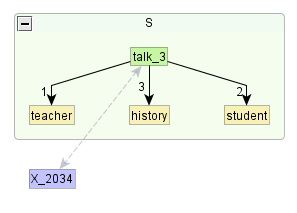
\includegraphics[width=0.4\textwidth, trim = {0cm 0cm 0cm 0cm},clip]{ch6/figs/root.png}
	\caption{Création de la racine à partir du noe{}ud dominant}
	\label{deroulement0}
\end{figure}

\subsection{Sélection du patron de régime dans le lexicon}:
Ensuite, une fois que le noe{}ud dominant est lexicalisé, la règle \emph{actant\_gp\_selection} est déclenchée. Celle-ci permet à GenDR de récupérer les traits encodés dans gp. Puis, à l'intérieur de gp, il y a les traits \texttt{id} et \texttt{dia}. Ces traits sont donc récupérés par la règle et apposé sur le noe{}ud racine. La racine est maintenant contrainte d'utiliser le patron de régime x si la diathèse qu'elle a correspond aux mêmes actants demandés par la structure d'input.

\begin{figure}[htb]
	\centering
	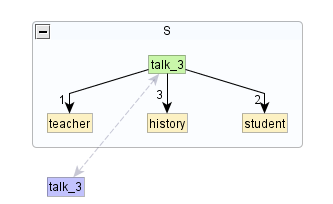
\includegraphics[width=0.4\textwidth, trim = {0cm 0cm 0cm 0cm},clip]{ch6/figs/selectiongp.png}
	\caption{Application de la règle actant\_gp\_selection}
	\label{deroulement1}
\end{figure}

\subsection{Application de la règle actancielle: \emph{actant\_gp\_ijk}}
À l'étape précédente, le noe{}ud \lex{talk\_3} se fait imposer les restrictions suivantes: une paire identifiant de gp et diathèse. Ces traits sont essentiels à l'application des règles actancielles. La règle actant\_gp\_ijk est sélectionnée lorsque la diathèse précise qu'il y a trois actants sémantiques. Il faut aussi que les actants sémantiques que la diathèse précise se retrouve dans la structure sémantique donnée. Sinon, aucune règle actancielle n'est appliquée et la réalisation s'interrompt laissant une racine comme output. 

Ce mécanisme est nouveau puisque dans l'ancienne version de GenDR, le système analysait liaison actancielle individuellement, puis faisait correspondre cet liaison sémantique à une relation syntaxique. Cela se traduisait par la création d'un arc entre la racine et un noe{}ud vide et on y ajoutait des contraintes sur ce noe{}ud simultanément. La version actuelle de GenDR ne fonctionne plus ainsi. Une fois que le gp est sélectionné, on confirme à l'aide du trait dia quel règle actancielle il faudra choisir. Dans notre exemple, ce sera celle-ci puisqu'elle correspond à un gouverneur sélectionnant trois actants.

La règle actant ijk, crée 3 arcs en partance talk\_3 au bout desquels se trouvent des noe{}uds vides sans contraintes. Elle s'occupe aussi du passage des arcs sémantiques à syntaxique. Le patron de régime qui nous concerne est le suivant: \lstinline!gp = { id=NP_V_PP_about_topic_PP_to_co_agent dia=132 }!. On peut y lire que la diathèse précise que le 1 actant sémantique reste le 1er actant syntaxique, mais que le deuxième actant syntaxique est le 3e sémantique et ainsi de suite. Elle crée donc les arcs syntaxiques à partir de ces informations et ils sont vides.

\begin{figure}[htb]
	\centering
	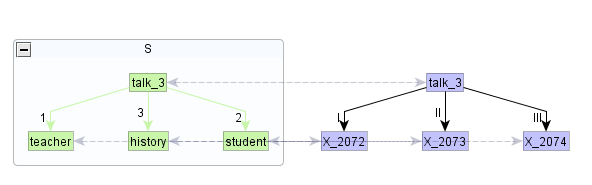
\includegraphics[width=1\textwidth, trim = {0cm 0cm 0cm 0cm},clip]{ch6/figs/actant_gp_ijk.png}
	\caption{Application d'une règle actancielle: actant\_gp\_ijk}
	\label{deroulement2}
\end{figure}

\subsection{Application des contraintes sur les noe{}uds}
Dans l'ancienne version de GenDR, la règle actancielle contraignait aussi les noe{}uds nouvellement créés en syntaxe. Notre système a dû créé une règle séparée de la règle actancielle pour des raisons d'efficacité. Nous avons ainsi créé une règle qui contraints chaque noe{}ud nouvellement créé à partir des informations demandées par le patron de régime pour chaque actant syntaxique. Bref, la règle récupère les restrictions sur les noe{}uds dans le gpcon tel qu'on le voit à la figure \ref{gpexemple}. La règle s'applique donc 3 fois puisqu'il y a trois noe{}uds vides. On a maintenant trois noe{}uds contraints.

\subsection{Lexicalisation des noe{}uds contraints}
Ensuite, on répète une règle de lexicalisation. Dans ce cas il s'agit de \emph{lex\_standard} puisque tous les sémantèmes figurent dans le semanticon et le lexicon. La règle s'applique trois fois car il y a trois noe{}uds. Puis la lexicalisation réussi à chaque fois puisque ces lexèmes satisfont les contraintes imposées aux noe{}uds.
\begin{figure}[htb]
	\centering
	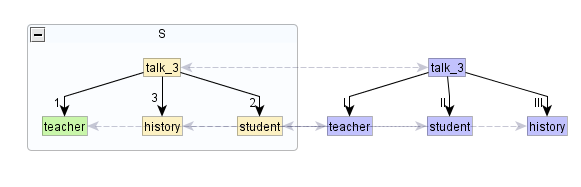
\includegraphics[width=1\textwidth, trim = {0cm 0cm 0cm 0cm},clip]{ch6/figs/lex.png}
	\caption{Applications d'une règle de lexicalisation: lex\_standard}
	\label{deroulement3}
\end{figure}

\subsection{Application de la règle \emph{actant\_gp\_selection}}
Finalement, la règle \emph{actant\_gp\_selection} s'applique encore, mais cette fois-ci pour les lexèmes \lex{teacher},\lex{student} et \lex{history}. Cette règle récupère leurs traits gp.id et gp.dia. Comme ce sont tous des noms communs, ils héritent du gp par défaut de la classe nominale id=NP dia=1 (nous n'avons pas plus d'information sur les patrons de régime des noms compte tenu que VerbNet se spécialisait dans les verbes, mais il existe d'autres ressources parmi celles que nous avions mentionnées qui pourrait combler cette lacune. C'est pourquoi nous n'avons que un gp pour les noms et qu'il est doté d'une diathèse simple permettant de faire la relation complément du nom). encore puisque ces nouveaux noe{}uds lexicalisés déclenchent l'application de la règle. Dès qu'un x a un gp, on va le repêcher, même si on s'en sert pas après. Si l'un d'entre eux avait eu un complément du nom, alors la sélection du gp aurait prouvé son utilité. C'est une application systématique.

Bref, l'application de toutes ces règles à notre input(figure \ref{input-text}) a permi son arborisation. Nous décrirons dans la section suivante le passage vers la structure syntaxique de surface.

\subsection{Lexicalisation de surface}
La première étape est de lexicaliser en surface les lexèmes profonds. Cette règle récupère aussi la partie du discours de surface de l'entrée lexicale. Le procédé est le même que nous avons vu au chapitre \ref{chapgendr}.

\subsection{Règles actancielles de surface}
Une fois que les lexèmes sont réalisés en surface, les règles actancielles de surface sont déclenchées. Trois règles actancielles de surface seront appliquées puisqu'il y a 3 arcs de dépendances (I, II et III) à réaliser. Concrètement, la règle récupère la valeur du trait \texttt{rel}. 

Donc, la règle synt\_subj est déclenchée et le système récupère l'information sur l'actant syntaxique qui possède le trait texttt{rel}. Comme nous avons choisi l'arborisation à partir du gp \emph{NP\_V\_PP\_to\_co\_agent\_PP\_about\_topic}, le système récupère l'information suivante: \lstinline! I={rel=subjective dpos=N}!. Le produit est le changement d'étiquette de la relation pour la valeur \texttt{subjective}.

Simultanément, la règle \emph{synt\_actant\_prep} est déclenchée une première fois pour faire la correspondance entre l'arc syntaxique qui lie \lex{talk\_3} et \lex{history}. La règle récupère ainsi le code suivant: \lstinline! II={rel=oblique dpos=N prep=about}!. Cela signifie que l'actant syntaxique II correspond à la relation \texttt{oblique} en RSyntS. Cette règle est déclenchée car l'un des actants syntaxiques s'expriment en syntaxe de surface à l'aide d'une préposition (une lexie fonctionnelle). Cela a pour incidence que le noe{}ud où profond de \lex{history} se scinde en deux afin que la préposition \lex{about} face le pont entre le verbe et l'objet indirect qu'il sélectionne. Ce phénomène est illustré par la figure~\ref{deroulement4}. 

Cette règle se déclenche une seconde fois pour traiter l'actant syntaxique III \lex{students}.

\subsection{Règles des déterminants}
Finalement, la règle det\_def réalise les déterminants qui doivent apparaître en syntaxe de surface. Ceux-ci correspondent aux traits que nous avions encodés dans l'input de départ. Seul \lex{teacher} et \lex{student} gouverneront des déterminants puisque leurs représentations sémantiques demandaient que les noe{}uds soit définis d'une certaine manière en syntaxe de surface. La règle de déterminant réalise \lex{the} lorsque c'est défini et \lex{a} lorsque le noe{}ud est marqué comme indéfini. Il s'agit d'une règle propre à l'anglais.
\begin{figure}[htb]
	\centering
	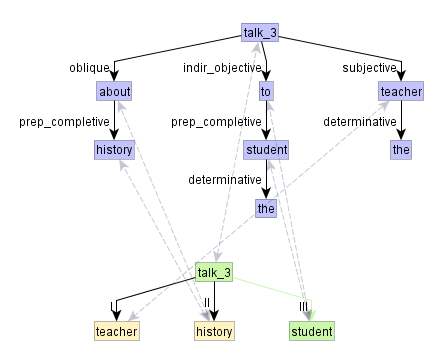
\includegraphics[width=0.5\textwidth, trim = {0cm 0cm 0cm 0cm},clip]{ch6/figs/ssynt.png}
	\caption{Applications des règles actancielles et réalisation des lexies fonctionnelles}
	\label{deroulement4}
\end{figure}
Cela met fin à notre chapitre implémentation. Nous passerons donc à la phase d'évaluation pour vérifier si notre système performe tel que nous l'avions prévu.